\subsubsection{\stid{1.12} Runtime System for Application-Level Power Steering on Exascale Systems} 

\paragraph{Overview} 
Power remains a critical constraint for Exascale. As we design supercomputers at larger scales, power becomes an expensive and limited resource. Inefficient management of power leads to added operational costs as well as low scientific throughput. Although hardware advances will contribute a certain amount towards achieving high energy efficiency, they will not be sufficient, creating a need for a sophisticated system software approach. Significant advances in software technologies are thus required to ensure that Exascale systems achieve high performance with effective utilization of available power. Distributing available power to nodes while adhering to system, job and node constraints involves complex decision making in software. 

The ECP PowerSteering project is developing a \emph{job-level} power management runtime system that will optimize performance of Exascale scientific applications transparently under power and/or energy constraints. Existing research efforts, including Conductor and Adagio, are being actively integrated into Intel's GEOPM runtime system, an ongoing open source effort led by Intel. This integration expands GEOPM's capabilities with the latest research while providing a production-grade, industry-supported open source solution. By developing new platform plugins, this project also supports upcoming target platforms and paradigms for ECP beyond the Intel architectures, and incorporates task-based programming models such as Legion. By being both configurable and cross-platform, GEOPM will help applications achieve maximum performance under a power constraint. 

This project is essential for ECP because it enables Exascale applications to operate safely with optimal performance under power and energy constraints. This project is also essential for building a sophisticated hierarchical software stack proposed by the ECP Argo and ECP Flux projects. Additionally, the project fulfills an essential need for ECP by enabling vendor and academic collaborations that provide for accelerated adoption of best practices and better interoperability at scale.  By leveraging the GEOPM software developed in this project, compute centers can safely operate under power and energy constraints while maximizing performance and scientific throughput. 


\paragraph{Key Challenges}
Power management in software is challenging due to the dynamic phase behavior of applications, processor manufacturing variability, and the increasing heterogeneity of node-level components. While several scattered research efforts exist, a majority of these efforts are site-specific, require substantial programmer effort, and often result in suboptimal application performance and system throughput. Additionally, these approaches are not production-ready and are not designed to cooperate in an integrated manner. A holistic, generalizable and extensible approach is still missing in the HPC community, and a goal for the ECP PowerSteering project is to provide a solution for this technology gap. 

Another set of challenges come from portability issues. Existing solutions are targeted toward specific Intel microarchitectures as well as programming models. Additionally, some of the existing solutions  violate the specified power budget before reaching a steady state, resulting in power fluctuations as well as unsafe operation. As part of this project, we strive to provide portability as well as safe operation using both hardware-level and application-level information for adaptive configuration selection and critical path analysis.

\paragraph{Solution Strategy}
Our solution is to develop a job-level runtime system (Intel GEOPM) that can operate transparently to user applications, and can also cooperate with HPC resource managers and node-level tools. We are taking a two-pronged approach. First, we are working toward consolidating existing research efforts from the community to develop high-quality plugins for GEOPM that can be deployed at Exascale. In parallel, we are developing new algorithms in GEOPM to address other challenges such as heterogeneity and variation. While GEOPM already provides some baseline algorithms, the existing capabilities are not programmer transparent and not sufficient for Exascale. Our advanced algorithms analyze critical paths of scientific applications transparently, balance power between different components intelligently, and provide mechanisms to capture fine-grained application semantics through Caliper. Additionally, these advanced algorithms will support non-Intel architectures such as IBM/NVIDIA and novel task-based programming models such as Legion. We also intend for GEOPM to be a part of a holistic power management stack that does dynamic, hierarchical power management and works closely with resource managers such as SLURM or Flux.  In order to accomplish portability and smooth integration, we are closely collaborating with ECP Argo and ECP Flux projects, with University of Arizona, and with Intel and IBM. 

\paragraph{Recent Progress}
We achieved two milestones in September 2018. The first was to port GEOPM to a non-Intel architecture. We chose IBM Power9 (Witherspoon) architecture for this, which applies well to the Sierra/Summit systems. We developed a DVFS-based model for Intel GEOPM and leveraged NVIDIA's NVML library to create this port. We also studied the impact of basic telemetry and power capping, and helped identify power-related bugs in IBM OPAL firmware. Currently, we are working on extending \texttt{libvariorum} to support IBM Witherspoon. \texttt{Libvariorum} is a device-agnostic, vendor-neutral power management library which will be integrated into GEOPM in our next milestones. 

The second milestone involved integrating Legion with GEOPM and creating a new benchmark for evaluation. GEOPM calls were placed inside Legion source code because the default model is for a separate GEOPM process to be created, and the GEOPM calls use shared memory to talk to that process. While GEOPM works correctly with Legion in this way, it is unable to provide any benefit with dynamic power balancing due to Legion's inbuilt load balancer. As part of our next milestone, we are researching options to change the default mapper in Legion runtime itself, so we can benefit from power balancing and scheduling power intelligently. Releases were made separately for the two milestones on GitHub. We are now working on testing and evaluation of our framework with the new model and collecting new data on the Quartz cluster at LLNL as well as on \texttt{alehouse}, which is a IBM Power9 node that we purchased for our lab to provide for root and privileged access. 

We established the PowerStack community charter in June 2019, involving collaborators across multiple vendors (Intel, IBM, ARM, HPE, AMD), academic institutions (TU Munich, Univ. Tokyo, Univ. Bologna, Univ. Arizona), and national laboratories (Argonne National Lab).The goal for this team is to design a holistic, flexible and extensible concept of a software stack ecosystem for power management. PowerStack explores hierarchical interfaces at three specific levels: batch job schedulers, job-level runtime systems, node-level managers. Each level will provide options for adaptive management depending on requirements of the supercomputing site under consideration. Site-specific requirements such as cluster-level power bounds, user fairness, or job priorities will be translated as inputs to the job scheduler. The job scheduler will choose plugins to ensure compliance, with the primarily responsibility for managing allocations across multiple users and diverse workloads. Such allocations will serve as inputs to a fine-grained, job-level runtime system to manage specific application ranks, in-turn relying on vendor-agnostic node-level measurement and control mechanisms. The figure below presents an overview of the envisioned PowerStack.

\begin{figure}[t]
	\centering
	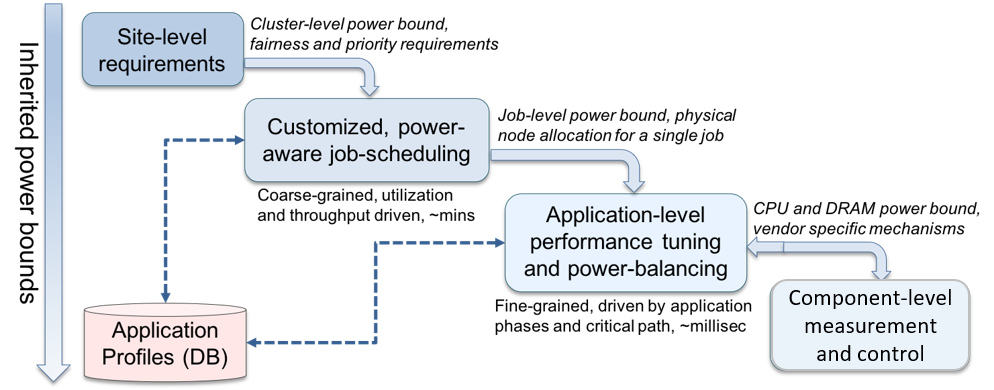
\includegraphics[scale = 0.7]{projects/2.3.1-PMR/2.3.1.12-Power-Steering/PowerStack_v2.png}
	\caption{Envisioned PowerStack}
	\label{fig:pstack}
\end{figure}

\paragraph{Next Steps}
We will continue our research and development work as planned toward the March 2019 milestones. More specifically, we are migrating to Intel GEOPM's new codebase, working on GPU power capping research, and enabling user-space access to power management on diverse architectures. We also continue to enhance our variation-aware and phase aware model with advanced machine learning and statistical techniques, and are working with Intel on understanding variation data from Theta. In the Legion space, we continue to explore dependency graphs and scheduling of dependency graphs in an intelligent, power-aware manner by creating a new mapper. We are also looking into S3D application code as part of our Legion power model  exploration. Lastly, we are looking into adding Spack support for installing GEOPM. 

